\documentclass{article}

\usepackage{amsmath}
\usepackage{balance}       % to better equalize the last page
\usepackage{graphicx}      % for EPS, load graphicx instead 
\usepackage[T1]{fontenc}   % for umlauts and other diaeresis
\usepackage{txfonts}
\usepackage{mathptmx}
\usepackage[pdflang={en-US},pdftex]{hyperref}
\usepackage{color}
\usepackage{booktabs}
\usepackage{textcomp}
\usepackage{multirow}
\usepackage{caption}
\usepackage{subcaption}

\begin{document}


\title{CS6850 Reaction Paper}
\author{Hangil Chung (hc685), Soobin Han (sh767)}
\date{March 23, 2018}

\maketitle


\section{Introduction}
Following the lectures on cascading networks, we read \textit{Maximizing the Spread of Influence through a Social Network} by Kempe, Kleinberg, and Tardos, and \textit{Mitigating Overexposure in Viral Marketing} by Abebe, Adamic, and Kleinberg. Both papers provide useful formulations of the seed selection problem in social networks. The nodes in these networks work as agents that propagate the effect of an "innovation," the subject of interest, to its neighbors. In our reaction paper, we first provide a review of the two papers and the strengths and weakness of each. Secondly, we go on to provide our own extension of the two papers. Specifically, we examine the problem of introducing stochasticity into the model provided in Abebe et al. and how one can choose the best initial seed node within clusters.

\section{Literature Review}
Both works present meaningful extensions to how the cascading network problem was first introduced in class. Whereas we first viewed tree-like cascading networks with some initial node (e.g. patient zero) to determine the growth of the "innovation," the problem formulations in both of these papers present us a family of optimization problems in which we select a set of several patient zeros to maximize the spread.

Kempe et al. begin by presenting two classes of problem formulation. The first, referred to as the Threshold problems, requires that a node \textit{v} is deterministically activated if the sum of the neighboring nodes' weights $b_{u,v}\in[0, 1]$ for each neighbor $v$ exceeds the activation threshold $\theta_u$. The General Threshold model extends the said model by allowing the activation function (formerly the sum of the neighboring nodes' weights) to be any monotone function with regards to the size of the active neighboring nodes. The second class of formulation is called the Cascading model, which more closely resembles the cascading network that we covered in class. Instead of the inactive target node $u$ being deterministically activated with sufficient activation value, each active neighboring node $v$ has one opportunity to activate $u$ with some predetermined probability $p_{u, v}$. Note here that $p_{u, v}$ is independent of the active neighboring nodes of $u$; in other words, the probability that the active neighbor $v$ activates $u$ is independent of the order in which $u$'s neighbors are activated. The generalized version of this formulation lifts this limitation by allowing the activation probability between a pair of nodes to depend on the currently active set of nodes of the target node. In other words, each active node $v$ now gets one opportunity to activate an inactive neighboring node $u$ with probabilty $p_v(u, S)$, where $S$ is the current set of active neighbors of $u$.

Theorems 2.1 and 2.2 in this paper quickly show that there does not exist a polynomial-time solution for determining the seed set with optimal resulting active node set. However, the paper present some approximation promises that can be met as long as the formulation of the problem satisfy several criteria. For example, Kempe et al.'s show that the Submodular Threshold model, in which the probability function $f_v(u, S)$ of a target node $v$ from a neighboring active node $u$ is submodular with respect to the set of active nodes of $v$, can be approximated to the factor of $1-1/e$. In other words, as long as $$f_v(u, S\cup{w}) - f_v(u, S) \geq f_v(u, T\cup{w}) - f_v(u, T)$$, where $S \supseteq T$, an approximation with guaranteed accuracy of the factor of $1-1/e$ can be computed in polynomial-time. Furthermore, the paper shows that the Submodular Threshold model is equivalent to the Decreasing Cascade model, again a special case of the Cascade model, in which the probability of target node $u$'s activation is non-increasing with respect to the size of the set of nodes that attempted to influence $u$ in the past. This equivalence relationship provides a good flexibility in formulating real world problems. While it may seem limiting that the approximability guarantee is only valid for the the two special cases, the submodularity of the activation functions - which are key factors in providing the guarantee - allows for a natural translation of the real life occurrence of diminishing margin of return on the activation attempts into a well contained mathematical function, meaning that the two "special" cases well model real life examples.

Utilizing the submodulartiy of the activation function, the paper introduces a greedy hill climbing algorithm for selecting the seed set. An array of experiments on simulated networks show that the hill climbing approach does indeed perform better (i.e. result in a larger resulting active node set) than other intuitive heuristics, such as selecting nodes with high degree or selecting "central" nodes.

While Kempe et al.'s  work presents a rich breadth of varying seed set problem formulations, one weakness is that the means of evaluating a seed set is very limited. The effectiveness of various heuristics is measured solely on the size of the resulting set of active nodes. While such evaluation may have been a good starting point for traditional problem space of seed selection, it does leave a considerable room for further exploration with evaluation functions. 

Abebe et al. present a natural extension of the works shown in Kempe et al., most notably by introducing a more interesting means to evaluate a seed set. Taking viral marketing as an inspiration, they suggest an interesting modification to the Linear Threshold model suggested in Section 2 of Kempe et al. by 1) introducing a new "criticality" parameter that indicates the attractiveness of a product and 2) the concept of "overexposure." Whereas the quality of a seed set in Kempe et al. was determined solely by the number of nodes that the activation process would eventually achieve, the new model in this paper introduced two types of nodes, the first of which contribute positively to the final payoff of the spread and the other negatively. This addition now requires us to evaluate the solution of the problem not in terms of the size of the resulting influenced nodes but a more specific payoff function that reflects how much the innovation benefits from reaching the "good" nodes and is hurt from reaching the "bad" nodes.

The paper also presents two, "unbudgeted" and "budgeted," cases of this problem. The first, unbudgeted problem allows us to select a seed set of any arbitrary size, whereas the second, budgeted, problem limits the size of the seed set to at most k. There exists a convenient reduction of the unbudgeted problem into an instance of the min-cut problem in a flow network, to which there exists various polynomial time solutions. However, we are shown that the budgeted problem is NP-complete, as we can create an instance of the clique problem which is also NP-complete. Simulations on sample networks with parameters drawn from various distributions verify that the optimal solution of the unbudgeted case do in fact return higher payoffs compared to several other seed sets based on other heuristics.

One aspect of Abebe et al.'s problem formulation that we thought was lacking was the introduction of stochasticity. While Kempe et al.'s work introduces the possibility of probabilistic activations through the Cascade Model, all the models presented by Abebe et al. assume a deterministic activation once the thresholds are met. While this formulation does lead to a nice polynomial time solution for the unbudgeted problem, it shows little resemblance to a real life social network where a sufficient number of contacts do not guarantee an activation of a node. 




\section{Extension: Introducing Stochasticity}

In this section we consider the model proposed in Abebe et al., when introducing stochasticity into the edge propagations. More specifically, we saw that under the unbudgeted regime, the problem of finding an optimal seed set to advertise can be solved optimally in polynomial time. Further, we saw the solution consisted of choosing a subset of clusters to include, and once having chosen the clusters, choosing any single canonical node within the cluster to be its representative seed agent. The reason the model can choose an arbitrary seed node within clusters is because the model assumes that agents always propagate the advertisement to all neighbors as long as the agent accepts the product (i.e. edge propagation has probability 1). In the following discussion, we break this assumption and instead consider the case where every agent has probability $p$ of propagating the advertisement to its respective neighbors. Once this stochasticity is introduced into the system, selecting the seed node within a cluster is no longer trivial. In this section we will focus on how to choose this seed node within clusters.

Furthermore, in our model, we will no longer consider what subsets of clusters to include (this has already been solved in Abebe et al.) and instead focus on which seed node to select within a cluster. Thus our model will consider the following: given a cluster of nodes consisting of interior and exterior nodes, which add and subtract value respectively, what is the optimal single seed node. In the following subsections, we will introduce which data sets we used, the evaluation metric used to compare between heuristics, define several heuristics and provide the results. 

\subsection{Data Set and Evaluation Metric}

The data set we used comprises of an email network from a large European research institution (found on the Snap database: 'email-Eu-core network'). The network consists of 1005 nodes and 25571 edges. Each node in the network represents an email user, and an undirected edge exists between two users if they have exchanged emails. After analyzing the network, we found the network to be highly connected. When we fixed the product "appealing" parameter $\theta$ and found the clusters within the network we found that, due to the highly connected nature, there was often only one single large cluster and many very small clusters for almost all parameters of $\theta$.  Thus we focused our analysis on only the single largest cluster. 

Thus formally let us define graph $G$ to be the email network. Then for a parameter $\theta$ we can find the resulting clusters formed. Let us define $C_{\theta}$ to be the largest cluster. Then to account for the randomness, we will run $N$ number of iterations, where each iteration chooses for each edge whether or not to include it into the final cluster, with probability $p$. Let us define $C_{\theta}^i$ to be the cluster graph on the $i^{th}$ iteration. In our analysis we set $N=100$. 

Then given a particular $C_{\theta}^i$ and a seed node $v_{\theta}^i$, we will use an evaluation metric similar to that used in Abebe et al. and define the total payoff for this cluster instance to be the number of interior nodes reachable plus the number of exterior nodes \textit{unreachable} (i.e. we award a point for every interior node reachable and every exterior node unreachable). We add the number of exterior nodes unreachable, rather than subtract those reachable simply to keep the score purely positive. Then the total average payoff $\delta_{\theta}$ for a particular heuristic is the average of the payoffs across $N$ iterations. Formally, if we define $A_{v_\theta}^i$ and $B_{v_\theta}^i$ to be the interior and exterior node sets respectively reachable and unreachable from seed node $v_{\theta}^i$, then the average payoff is defined to be:

\begin{equation}
\delta_{\theta} =\frac{1}{N} \sum_{i=1}^{N} |A_{v_\theta}^i| + |B_{v_\theta}^i| 
\end{equation}

\subsection{Heuristics}
In our analysis we provide four different heuristics.
\\ \\
\textbf{Random} \\
This heuristic is the most basic and baseline heuristic. This policy simply choses at random a seed node from the set of interior nodes and serves as the baseline policy with which to compare other heuristics.
\\ \\
\textbf{Highest-Degree Interior Node} \\
This heuristic chooses from the set of interior nodes, the node which has the highest degree when considering only other interior nodes. More specifically, the policy chooses the node within the interior nodes which has the most number of interior neighbors. The intuition behind this policy is that this node will have the highest initial propagation rate to other interior nodes.
\\ \\
\textbf{Farthest from Exterior} \\
This heuristic is based on the intuition that we want to avoid the "bad" exterior nodes. Thus the policy first calculates the expected minimum-distance between all pairs of points within the original cluster $C_{\theta}$, and chooses the seed node to be the node which has the largest average expected distance to exterior nodes. We use the term "expected distance" because we incorporate into our calculations the probability of reaching a node via the shortest path. Specifically, if the shortest-path to an exterior node is 3 (3 edges away), then the expected distance is defined to be $\frac{1}{p^3}$ to reflect the probabilities of each edge. Formally if we define $d_{i,j}$ to be the distance between node $i$ and $j$, and $B_{\theta}$ to be the set of exterior nodes in the $C_{\theta}$ cluster, then the seed node is chosen as follows:
\\ \\
\begin{equation}
\text{arg}\,\max\limits_{i}\  \frac{1}{|B_{\theta}|} \sum_{j \in B_{\theta}} \frac{1}{p^{d_{i,j}}}
\end{equation}
\\ \\
\textbf{Near-Far} \\
This heuristic combines our desire to be far from "bad" exterior nodes and desire to be near "good" interior nodes. Thus using the same expected minimum-distance between all points, the policy calculates for each node the sum of the distances to the good nodes minus the sum of the distances to the bad nodes, and chooses the node with the largest value to be the seed node. Formally, let us define $A_{\theta}$ to be the set of interior nodes, and the seed node is chosen as follows:
\\ \\
\begin{equation}
\text{arg}\,\max\limits_{i}\  \sum_{j \in A_{\theta}} \frac{1}{p^{d_{i,j}}} -  \sum_{j \in B_{\theta}} \frac{1}{p^{d_{i,j}}}
\end{equation}
\\ \\

\subsection{Results}
Here we present the results for the four heuristics when run across various $\theta$ and $p$ values. Particularly, we present results when $\theta \in \{0.2, 0.4, 0.6, 0.8\}$, and for $p \in [0,1]$. To maintain the same scale across varying $\theta$ values, we present the results in relative terms of proportion of optimal score achieved. More specifically, for a cluster the theoretical optimal score when all nodes are reachable is the number of interior nodes plus the number of exterior nodes. Obviously, this is not always actually possible, however it simply gives us an upper bound on the possible score and lets us present the results in relative scores.
 \begin{figure}
  \begin{subfigure}{\linewidth}
  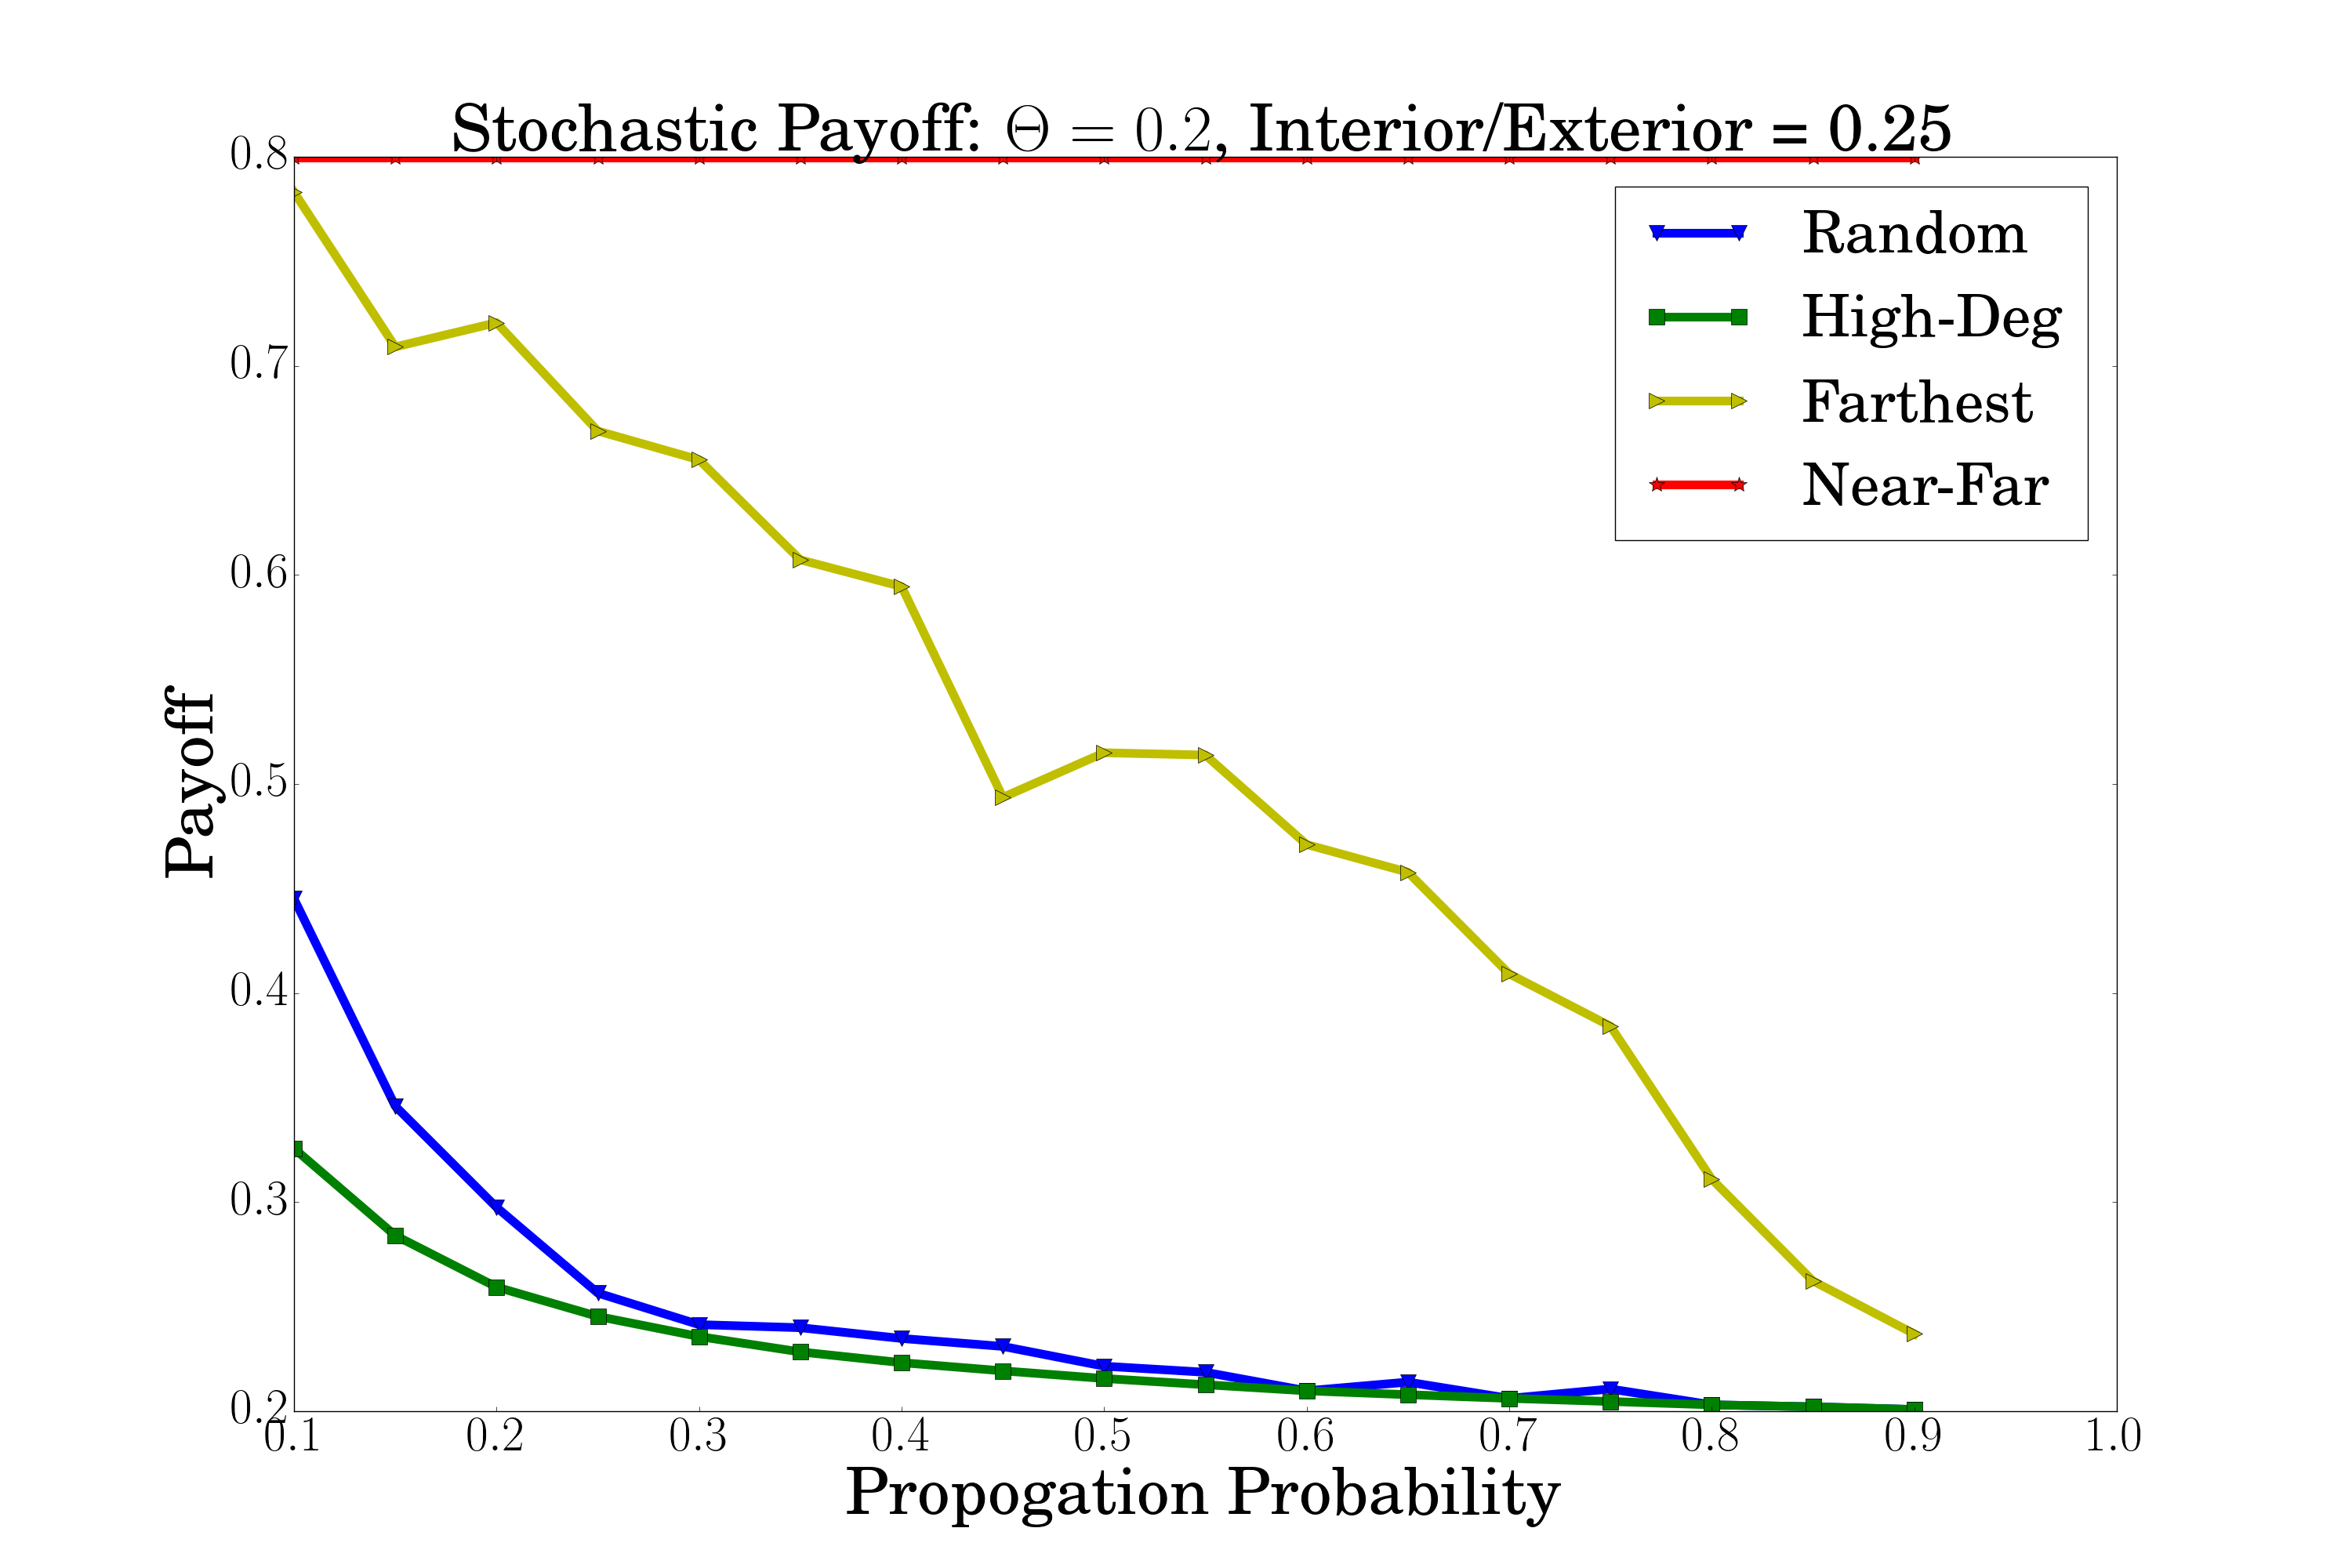
\includegraphics[width=1\textwidth]{../plots/actual/theta=2.png}
  \end{subfigure}\par\medskip
  \begin{subfigure}{\linewidth}
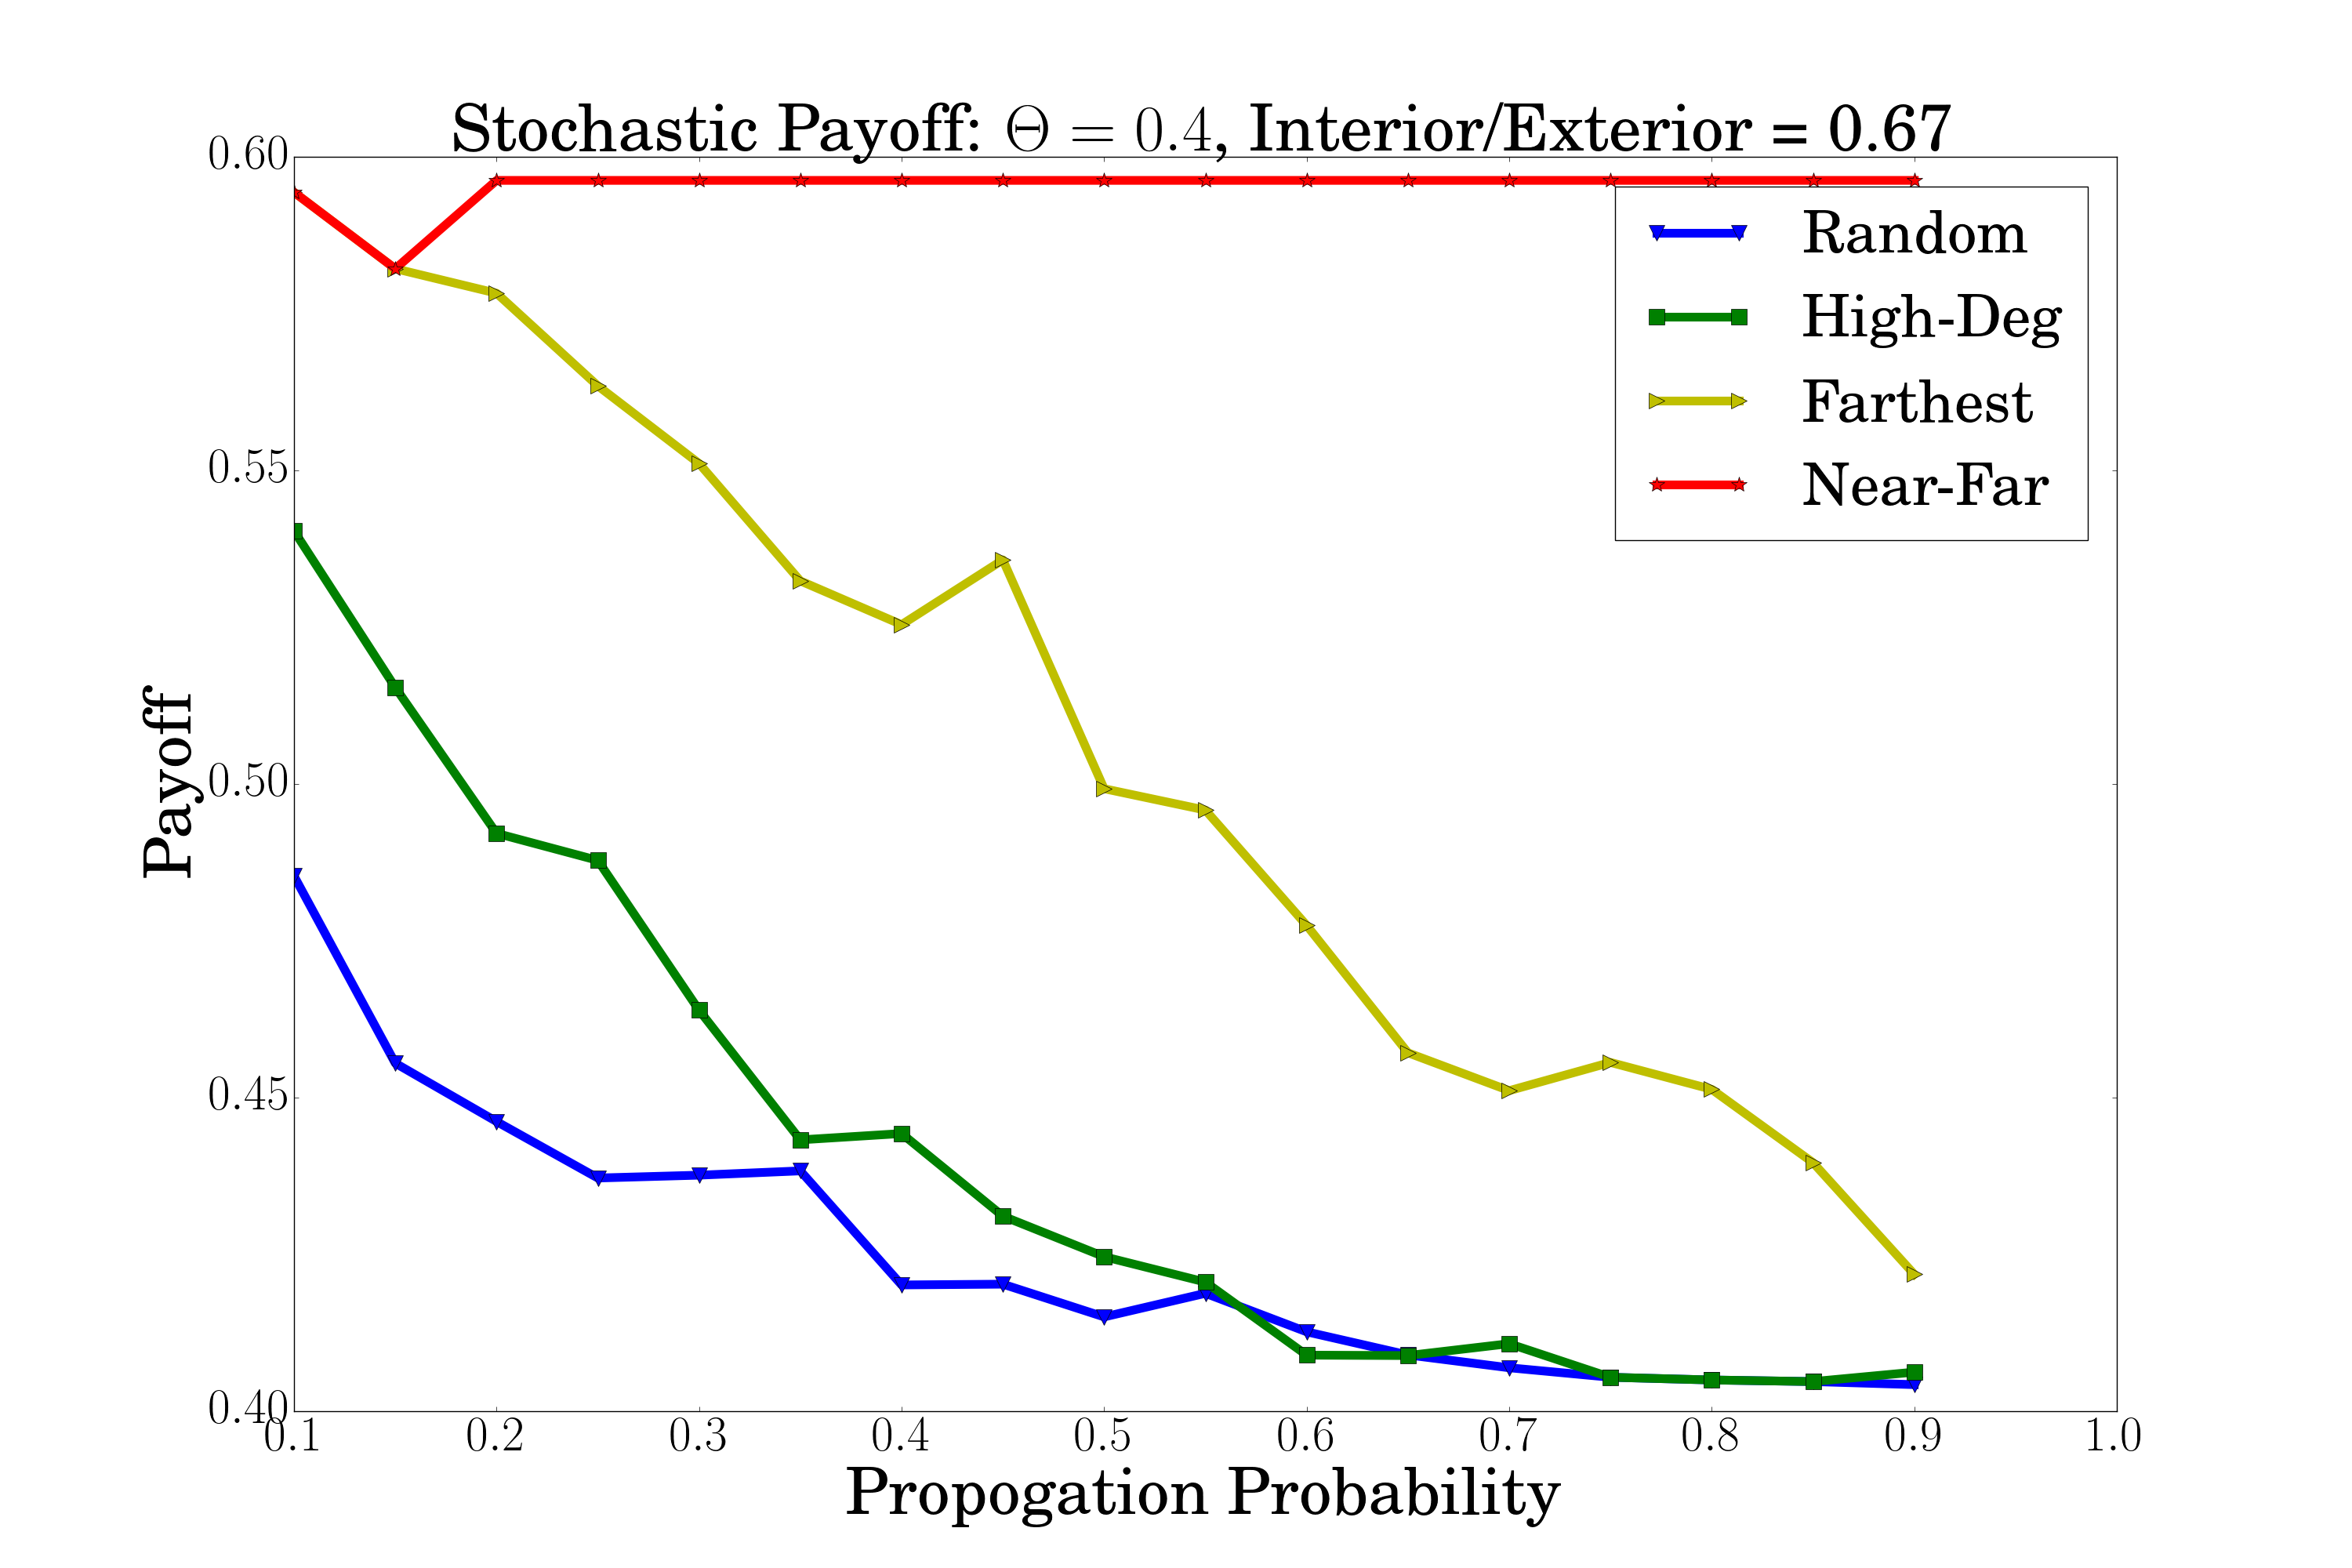
\includegraphics[width=1\textwidth]{../plots/actual/theta=4.png}
  \end{subfigure}\par\medskip
    \caption{Heuristic Results when $\theta$ < 0.5}
\end{figure}
  
  \begin{figure}
  \begin{subfigure}{\linewidth}
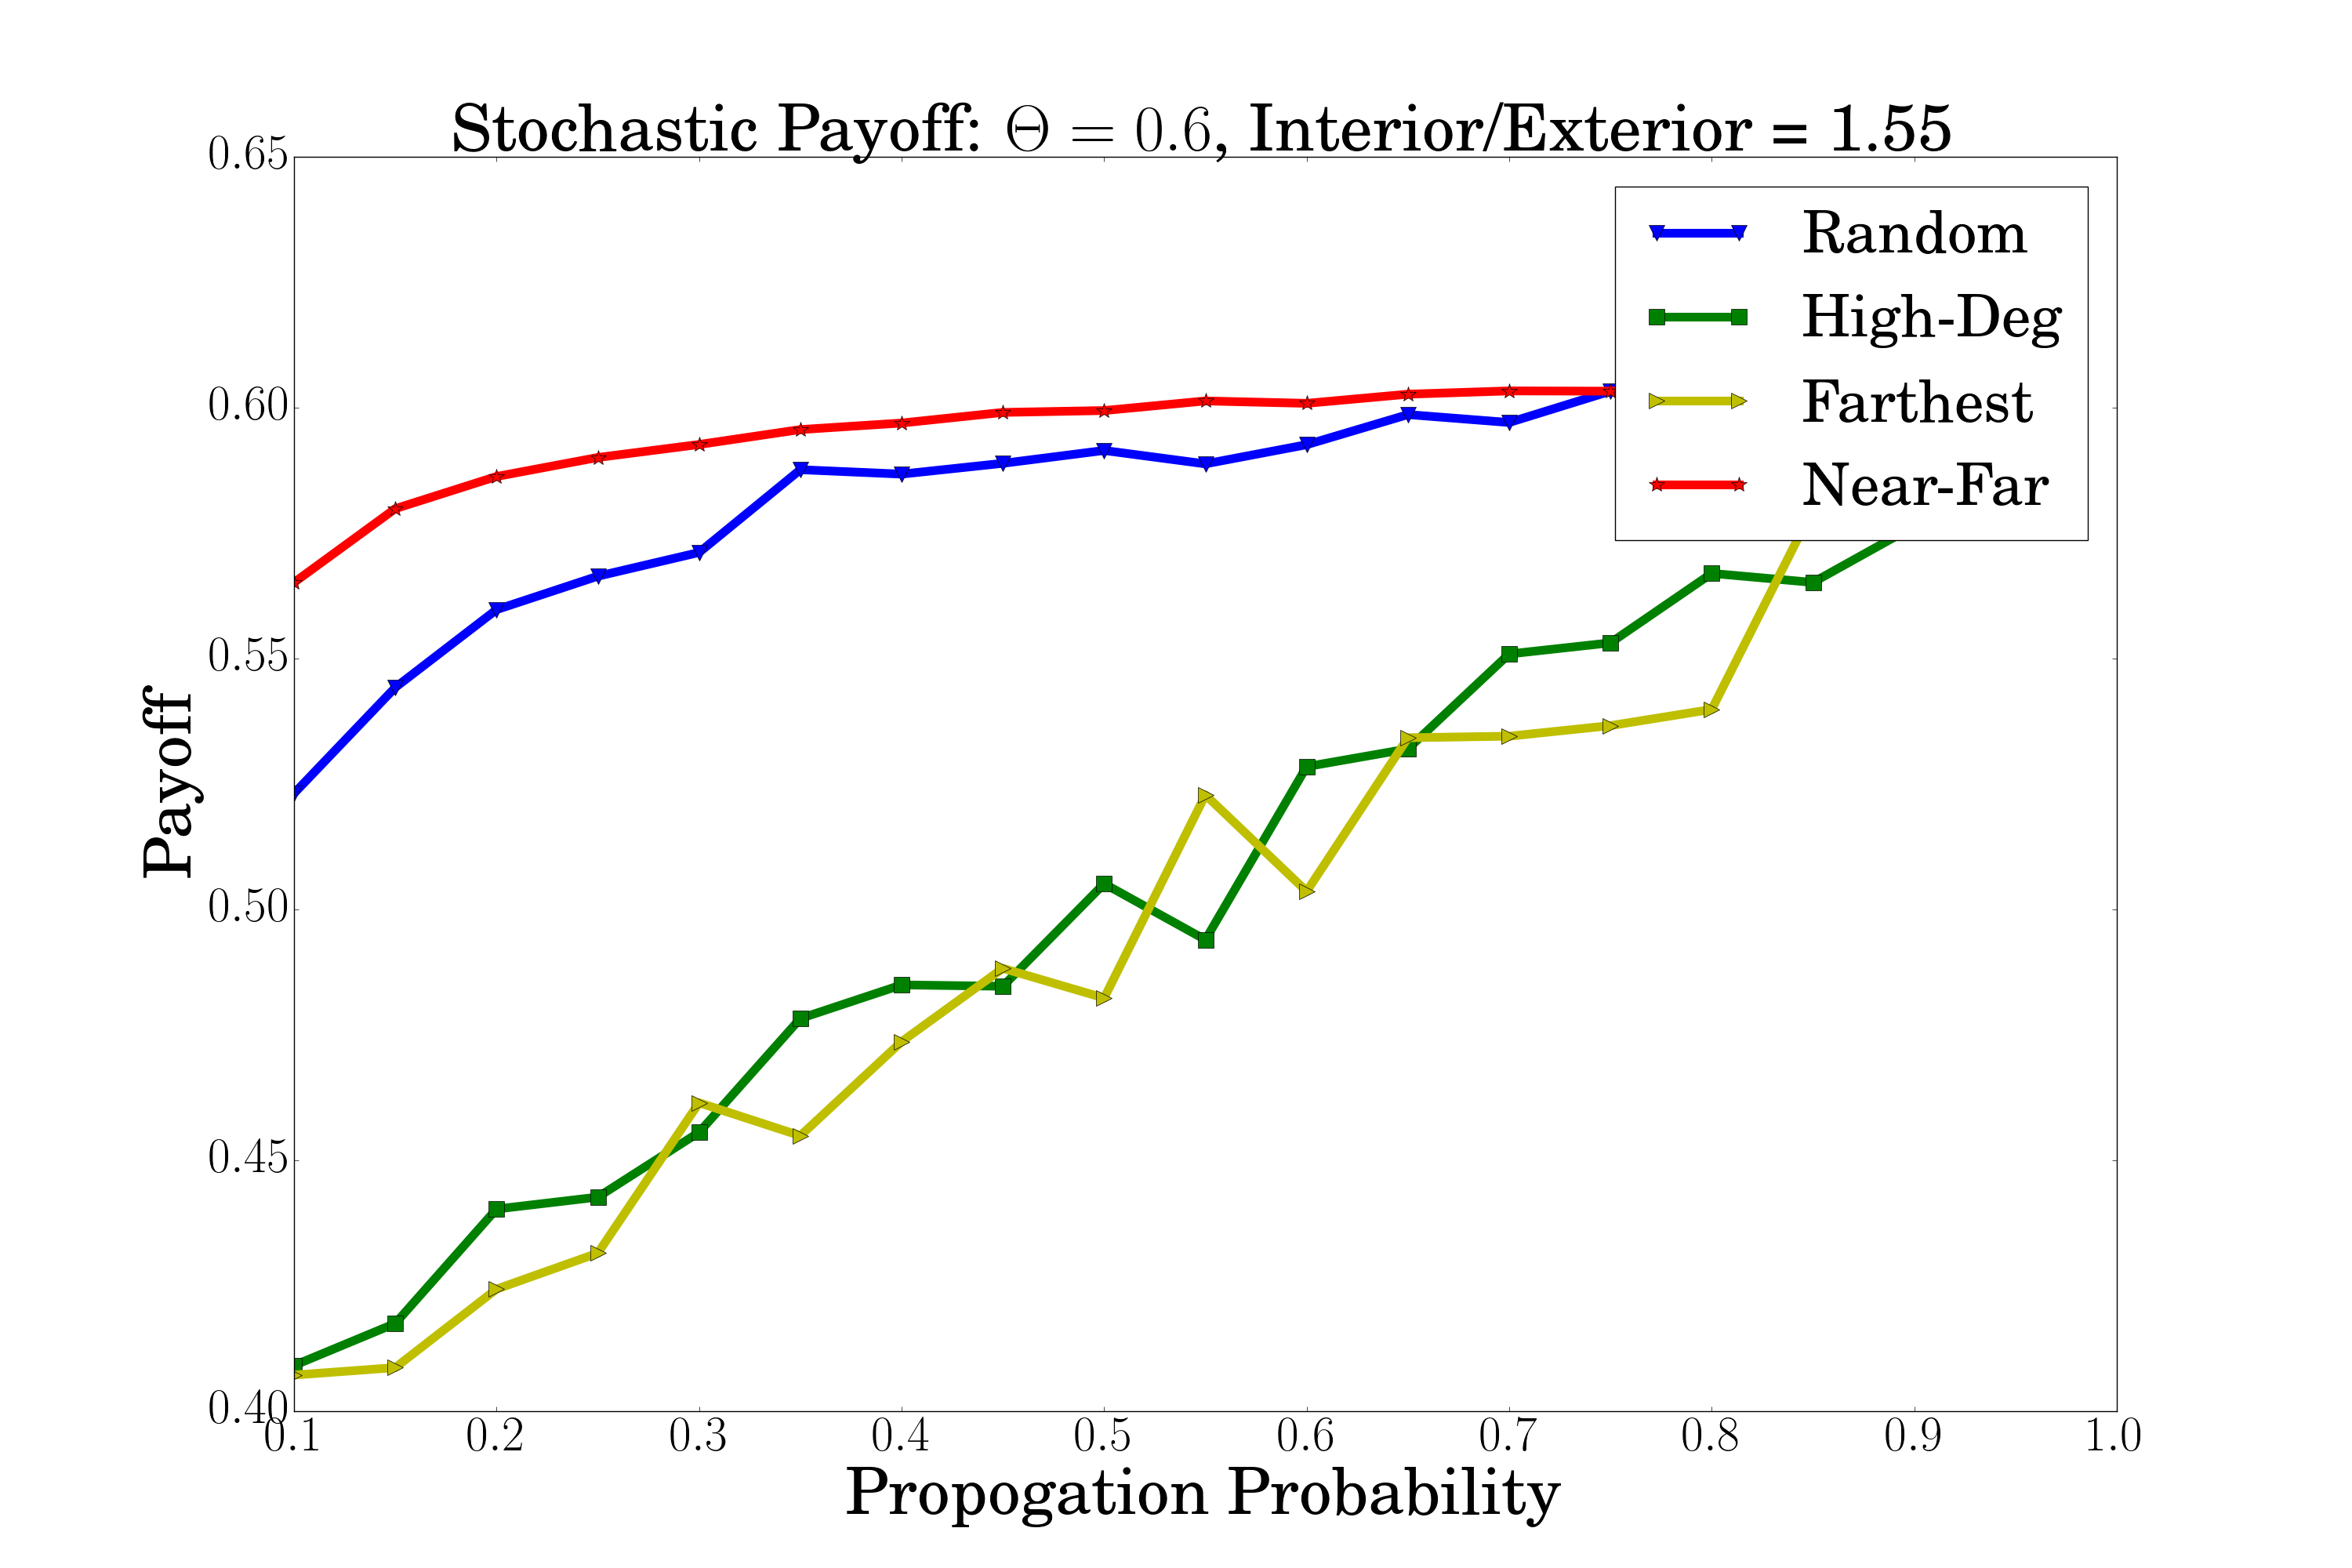
\includegraphics[width=1\textwidth]{../plots/actual/theta=6.png}
  \end{subfigure}
   \begin{subfigure}{\linewidth}
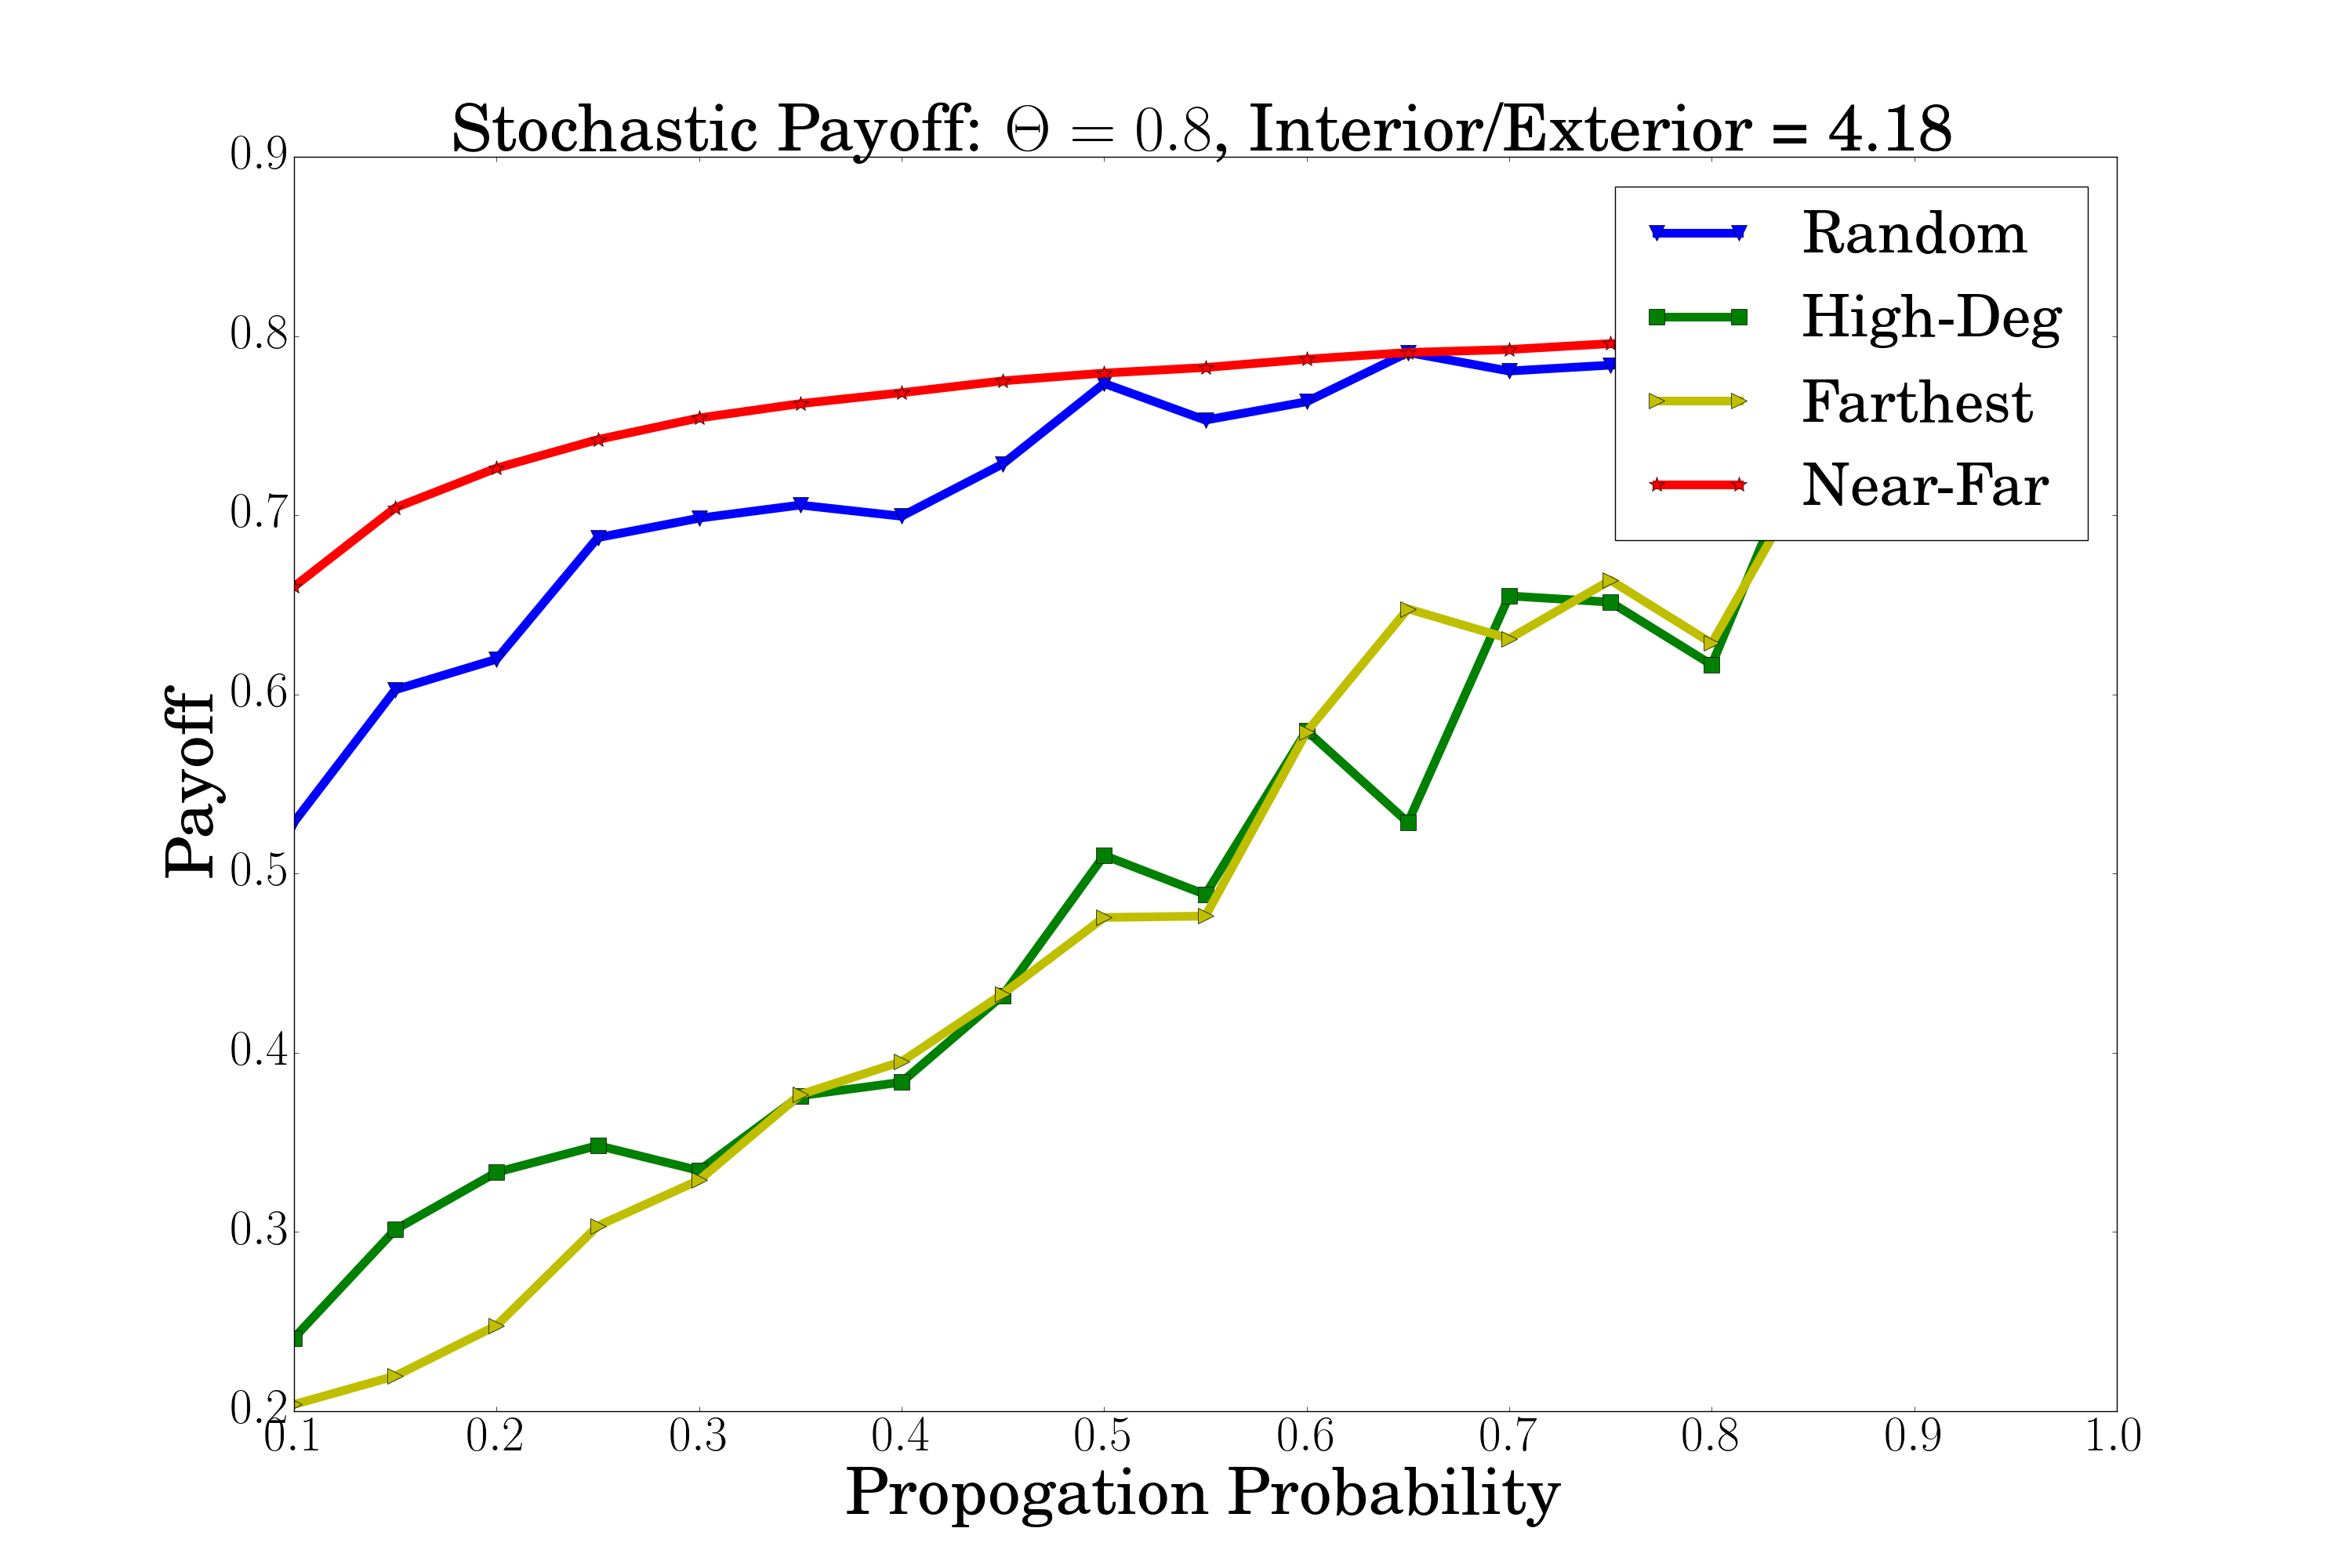
\includegraphics[width=1\textwidth]{../plots/actual/theta=8.png}
  \end{subfigure}
  \caption{Heuristic Results when $\theta$ > 0.5}
\end{figure}

The plots of the results are shown in Figures 1 and 2. Figure 1 shows the regime when $\theta < 0.5$ and Figure 2 shows the regime when $\theta > 0.5$. The $\theta$ values and perhaps more importantly the ratio of interior to exterior nodes are presented in the plot titles, and the x-axis indicates the varying probabilities of edge propagation and the y-axis is the relative performances. There are several interesting takeaways from the results discussed below.
\\ \\
\textbf{Random} \\
From looking at the figures, we can see that the random heuristic actually performs very well in the regime with high $\theta$ values. In fact, it beats out all heuristics except the Near-Far heuristic. However, in the regime with low $\theta$ values the random algorithm performs poorly. Intuitively this makes sense, especially when considering the interior/exterior ratios and the highly connected nature of the network. With high $\theta$ values, the ratio of interior/exterior nodes is high, and because the network is highly connected choosing a random node will perform quite well as chances are there are many connected interior nodes. On the other hand with low $\theta$ and interior/exterior ratios, choosing a random node performs poorly.
\\ \\
\textbf{Near-Far} \\ 
In all configurations, we find that the Near-Far heuristic performs the best of the heuristics presented. This makes sense, as this heuristic is the only one which reflects both our desire to be far from exterior nodes and close to interior nodes. What is interesting however, is that this heuristic seems to be the only policy which is not heavily influenced by the $p$ parameter. Particularly, we see all other heuristics performance being heavily influenced by $p$. However, the Near-Far policy seems largely unaffected by the changing $p$ parameter regardless of the $\theta$ value.
\\ \\
\textbf{ Increasing Edge Probabilities} \\
We see a trend that with increasing edge probabilities, the heuristics' performances all generally tend to perform more poorly when $\theta$ is less than 0.5, and tend to perform better when $\theta$ is higher than 0.5. Intuitively this makes sense. Under low $\theta$ regimes, there are more exterior nodes, and thus we prefer the edge propagation probabilities to be lower, while with high $\theta$ regimes we want the opposite. 
\\ \\
\textbf{ Farthest from Exterior} \\
In our results we find that the Farthest from Exterior heuristic performs quite well when both $\theta$ and $p$ is small. However, when either parameter increases the policy performs poorly. After further examination of why this is the case we found that the heuristic actually tends to find seed-nodes which are outlier nodes and have few edges. These outlier nodes are far from not only exterior nodes but also interior nodes. This explains why with increasing $\theta$, the heuristic performs poorly. 
\\ \\
\textbf{ Highest-Degree} \\
Interestingly, the highest-degree heuristic always performs poorly. From looking at the structure of the network, it seems that although the highest-degree nodes have an initial high propagation rate, it is not indicative of how much influence they will eventually have. 

\subsection{Conlcusion}
In our analysis of introducing stochasticity to the model we attempted to answer the question of how to choose the initial starting seed node within a cluster when edges have a propagation probability. Our results indicate that of the four heuristics presented, the Near-Far heuristic performs the best. However, this is obviously a very preliminary analysis of the problem and many other heuristics can be attempted. Furthermore, similar areas of work that could be explored is considering what happens when more than one seed is allowed to be chosen within each cluster. Similarly, a natural extension would be considering the same problem when each edge has different probabilities of propagation and how this affects the heuristics. 

\end{document}





